%%%%%%%%%%%%%%%%%%%%%%%%%%%%%%%%%%%%%%%%%%%%%%%%%%%%%%%%%%
%%
%% MARK: Title
%%
%%%%%%%%%%%%%%%%%%%%%%%%%%%%%%%%%%%%%%%%%%%%%%%%%%%%%%%%%%

\chapter*{\S B14. $1$-Forms on Half-Spaces}
\setcounter{footnote}{0}

%%%%%%%%%%%%%%%%%%%%%%%%%%%%%%%%%%%%%%%%%%%%%%%%%%%%%%%%%%
%%
%% MARK: Abstract
%%
%%%%%%%%%%%%%%%%%%%%%%%%%%%%%%%%%%%%%%%%%%%%%%%%%%%%%%%%%%

\begin{abstract}
  In this note we shall see that every differential $1$-form on the half-space $ H^n = [0,\infty[\, \times\, \RR^{n-1}$ is the restriction of a smooth $1$-form on $\RR^n$.
\end{abstract}

%%%%%%%%%%%%%%%%%%%%%%%%%%%%%%%%%%%%%%%%%%%%%%%%%%%%%%%%%%
%%
%% MARK: Content
%%
%%%%%%%%%%%%%%%%%%%%%%%%%%%%%%%%%%%%%%%%%%%%%%%%%%%%%%%%%%

This is an (almost) straightforward generalization of the proposition in ``$1$-Forms On The Half-Line'' from the previous article.
With a little rewriting,
this proof applies to all differential $k$-forms on half-spaces.

\begin{Article}{Differential $1$-form on half-space.}{}
  Let $ H^n = [0,\infty[\, \times\ \RR^{n-1}$ be the half $n$-space,
  equipped with the subset diffeology.
  Let $\alpha \in \DForms^1( H^n)$ be a differential $1$-form on $ H^n$.
  Then,
  there exists a smooth $1$-form $\bar\alpha$ defined on some neighborhood of $ H^n \subset \RR^n$ such that $\alpha = \bar\alpha \restriction H^n$.
\end{Article}

\begin{proof}
  Since $]0,\infty[\, \times\ \RR^{n-1} \subset [0,\infty[\, \times\ \RR^{n-1}$ inherits the usual smooth diffeology,
  we have
  $$%
    \alpha \restriction\ ]0,\infty[\, \times\ \RR^{n-1} = a(x,y) \, dx + \sum_{i=1}^{n-1} b_i(x,y) \, dy_i,
    $$%
  where $(x,y) \in ]0,\infty[\, \times\ \RR^{n-1}$ and $a, b_i \in \Cinfty(]0,\infty[\, \times\ \RR^{n-1},\RR)$.
  
  Now,
  let
  $$%
    \Sq_1 : (t,y) \mapsto (t^2,y),
    $$%
  then
  \begin{align*}
    \Sq_1^*(\alpha)_{(t,y)}(\delta t,\delta y) & = \alpha((t,y) \mapsto (t^2,y))_{(t,y)}(\delta t,\delta y) \\
    &  = A(t,y)\,\delta t + \sum_{i=1}^{n-1} B_i(t,y)\,\delta y_i,
  \end{align*}
  with $A, B_i \in \Cinfty(\RR^n,\RR)$.
  For all $t \neq 0$,
  $$%
    A(t,y) = 2t\, a(t^2,y) \quad \text{and} \quad B_i(t,y) = b_i(t^2,y).
    $$%
  Next,
  $\Sq_1^*(\alpha)$ is invariant under the map $(-1,1) : (t,y) \mapsto (-t,y)$,
  thus
  \begin{align*}
    \Sq_1^*(\alpha)_{(t,y)}(\delta t,\delta y)
    &= (-1,1)^*(\Sq_1^*(\alpha))_{(t,y)}(\delta t,\delta y) \\
    &= \Sq_1^*(\alpha)_{(-t,y)}(-\delta t, \delta y) \\
    &= A(-t,y)(-\delta t) + \sum_{i=1}^{n-1} B_i(-t,y)\,\delta y_i.
  \end{align*}
  Hence,
  $-A(-t,y) = A(t,y)$ and $B_i(t,y) = B_i(-t,y)$.
  In particular,
  $A(0,y)=0$.
  Therefore,
  there exists a smooth function $\underline{A} \in \Cinfty(\RR^n,\RR)$ such that $A(t,y) = 2t \underline{A}(t,y)$,
  for all $t\in \RR$.
  Thus,
  $a(t^2,y) = \underline{A}(t,y)$.
  Now, $\underline{A}$ is even in $t$,
  as are the $B_i$.
  We can then apply the Hassler Whitney theorem \cite[Theorem 1 and final remark]{Whi43} (see facsimile in lecture L8: ``Local Diffeology, Modeling''),
  stated as follows:
  
  \uline{Theorem. (Whitney)}~{\itshape If a smooth function $f(t,x)$ is even in $t$,
  $f(t,x) = f(-t,x)$,
  then there exists a smooth function $g(t,x)$ such that $f(t,x) = g(t^2,x)$.}
  
  Hence,
  there exists a smooth function $\underline{a}(x,y)$ such that $\underline{A}(t,y) = \underline{a}(t^2,y)$,
  and there exist $(n-1)$ smooth functions $\underline{b}_i$ such that $B_i(t,y) = \underline{b}_i(t^2,y)$.
  We then have,
  for all $t>0$,
  $a(t,y) = \underline{a}(t,y)$ and $b_i(t,y) = \underline{b}_i(t,y)$.
  
  Let us then define $\bar\alpha$ on $\RR^n$ by
  $$%
    \bar\alpha = \underline{a}(x,y) \, dx + \sum_{i=1}^{n-1} \underline{b}_i(x,y) \, dy_i.
    $$%
  The form $\bar\alpha$ is a smooth $1$-form defined on an open neighborhood of $ H^n$,
  and $\alpha \restriction\ ]0,\infty[\, \times\ \RR^{n-1} = \bar\alpha \restriction\ ]0,\infty[\, \times\ \RR^{n-1}$.
  Let us now prove that $\alpha$ and $\bar\alpha$ coincide on the whole $ H^n$.
  Since $\alpha$ and $\bar\alpha \restriction H^n$ are two differential $1$-forms on $ H^n$,
  it suffices to show that they take the same value on every smooth path.
  
  Let $\gamma$ be any path in $[0,\infty[\, \times\ \RR^{n-1}$.
  Let $\cO = \gamma^{-1}(]0,\infty[\, \times\ \RR^{n-1})$,
  which is open in $\RR$,
  and on this open subset $\bar\alpha(\gamma) = \alpha(\gamma)$.
  Hence,
  by continuity $\bar\alpha(\gamma) = \alpha(\gamma)$ on the closure $\overline \cO$ of $\cO$
  (since $\bar\alpha(\gamma)$ and $\alpha(\gamma)$ are smooth).
  %
  On the open subset $\RR - \overline{\cO}$,
  $\gamma$ takes its values in $\partial H^n = \{0\} \times \RR^{n-1}$;
  $\gamma \restriction \RR \setminus \overline{\cO}$ is a plot of the boundary $\partial H^n$.
  Let $i_2 : \RR^{n-1} \to \partial H^n$,
  $i_2(y) = (0,y)$.
  Then,
  $i_2^*(\alpha)$ and $i_2^*(\bar\alpha)$ are both $1$-forms on $\RR^{n-1}$.
  Let us prove that they coincide.
  On the one hand,
  $$%
    i_2^*(\bar\alpha)_y(\delta y) = \sum_{i=1}^{n-1} \underline{b}_i(0,y) \, \delta y_i.
    $$%
  On the other hand,
  note that
  $$%
    i_2 = \Sq_1 \circ i_2 : y \mapsto (0,y) \mapsto (0^2,y).
    $$%
  Thus,
  $i_2^*(\alpha) = i_2^*(\Sq_1^*(\alpha))$ and then $i_2^*(\alpha)_y(\delta y) = \Sq_1^*(\alpha)_{(0,y)}(0,\delta y)$.
  But,
  \begin{align*}
    \Sq_1^*(\alpha)_{(0,y)}(0,\delta y) &= A(0,y) \times 0 + \sum_{i=1}^{n-1} B_i(0,y) \, \delta y_i \\
    &= \sum_{i=1}^{n-1} \underline{b}_i(0,y) \, \delta y_i,
  \end{align*}
  since $B_i(t,y) = \underline{b}_i(t^2,y)$.
  Hence $\alpha$ and $\bar\alpha$ coincide on $\partial H^n$, and therefore $\bar\alpha(\gamma)$ and $\alpha(\gamma)$ coincide everywhere.
  
  Consequently,
  since $\bar\alpha$ and $\alpha$ coincide on all $1$-plots in $ H^n$, they coincide as $1$-forms \cite[\textsection\,6.37]{PIZ13},
  and thus
  $\alpha = \bar\alpha \restriction H^n$.
\end{proof}

\vfill
\centerline{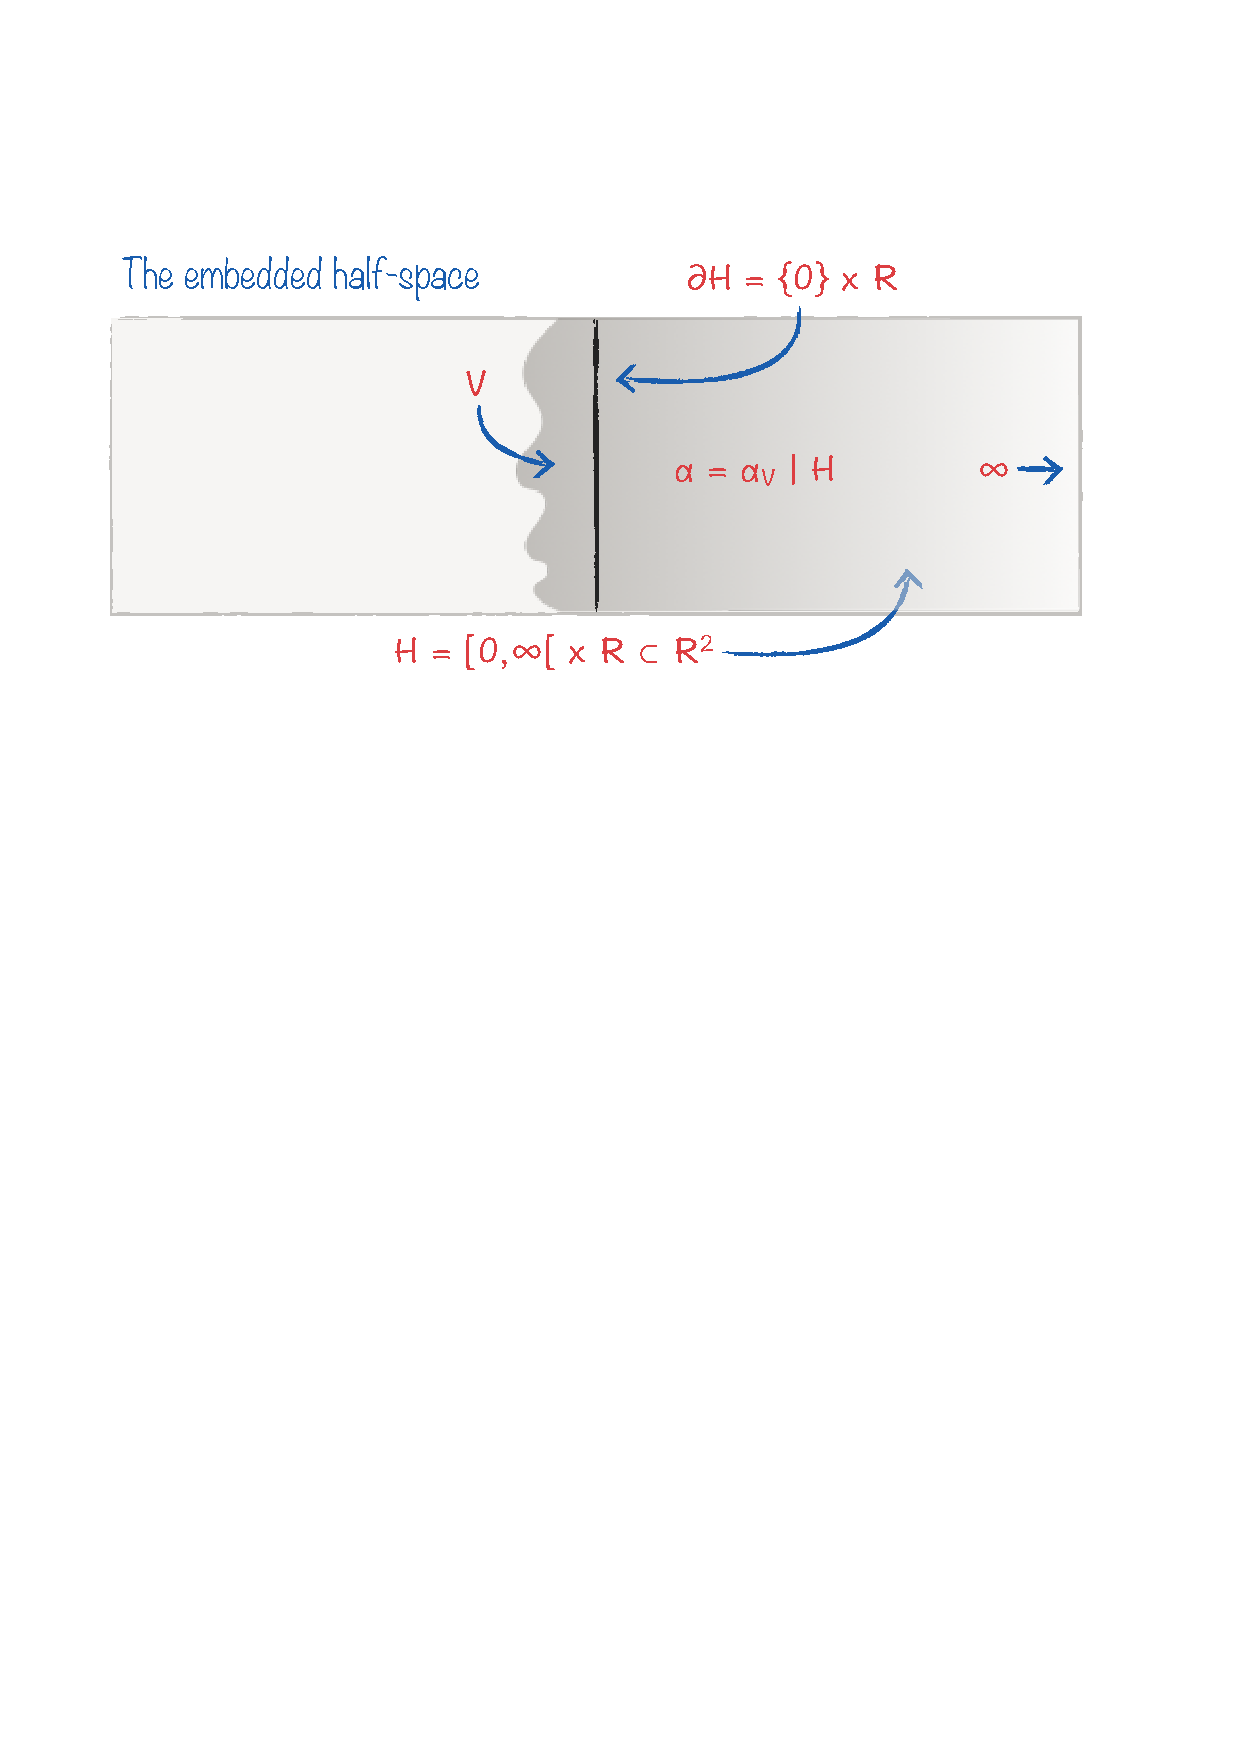
\includegraphics[width=1\textwidth]{Figures/Half-space.pdf}}
